% Options for packages loaded elsewhere
\PassOptionsToPackage{unicode}{hyperref}
\PassOptionsToPackage{hyphens}{url}
%
\documentclass[
  ignorenonframetext,
]{beamer}
\usepackage{pgfpages}
\setbeamertemplate{caption}[numbered]
\setbeamertemplate{caption label separator}{: }
\setbeamercolor{caption name}{fg=normal text.fg}
\beamertemplatenavigationsymbolsempty
% Prevent slide breaks in the middle of a paragraph
\widowpenalties 1 10000
\raggedbottom
\setbeamertemplate{part page}{
  \centering
  \begin{beamercolorbox}[sep=16pt,center]{part title}
    \usebeamerfont{part title}\insertpart\par
  \end{beamercolorbox}
}
\setbeamertemplate{section page}{
  \centering
  \begin{beamercolorbox}[sep=12pt,center]{part title}
    \usebeamerfont{section title}\insertsection\par
  \end{beamercolorbox}
}
\setbeamertemplate{subsection page}{
  \centering
  \begin{beamercolorbox}[sep=8pt,center]{part title}
    \usebeamerfont{subsection title}\insertsubsection\par
  \end{beamercolorbox}
}
\AtBeginPart{
  \frame{\partpage}
}
\AtBeginSection{
  \ifbibliography
  \else
    \frame{\sectionpage}
  \fi
}
\AtBeginSubsection{
  \frame{\subsectionpage}
}
\usepackage{amsmath,amssymb}
\usepackage{iftex}
\ifPDFTeX
  \usepackage[T1]{fontenc}
  \usepackage[utf8]{inputenc}
  \usepackage{textcomp} % provide euro and other symbols
\else % if luatex or xetex
  \usepackage{unicode-math} % this also loads fontspec
  \defaultfontfeatures{Scale=MatchLowercase}
  \defaultfontfeatures[\rmfamily]{Ligatures=TeX,Scale=1}
\fi
\usepackage{lmodern}
\ifPDFTeX\else
  % xetex/luatex font selection
\fi
% Use upquote if available, for straight quotes in verbatim environments
\IfFileExists{upquote.sty}{\usepackage{upquote}}{}
\IfFileExists{microtype.sty}{% use microtype if available
  \usepackage[]{microtype}
  \UseMicrotypeSet[protrusion]{basicmath} % disable protrusion for tt fonts
}{}
\makeatletter
\@ifundefined{KOMAClassName}{% if non-KOMA class
  \IfFileExists{parskip.sty}{%
    \usepackage{parskip}
  }{% else
    \setlength{\parindent}{0pt}
    \setlength{\parskip}{6pt plus 2pt minus 1pt}}
}{% if KOMA class
  \KOMAoptions{parskip=half}}
\makeatother
\usepackage{xcolor}
\newif\ifbibliography
\usepackage{longtable,booktabs,array}
\usepackage{calc} % for calculating minipage widths
\usepackage{caption}
% Make caption package work with longtable
\makeatletter
\def\fnum@table{\tablename~\thetable}
\makeatother
\usepackage{graphicx}
\makeatletter
\def\maxwidth{\ifdim\Gin@nat@width>\linewidth\linewidth\else\Gin@nat@width\fi}
\def\maxheight{\ifdim\Gin@nat@height>\textheight\textheight\else\Gin@nat@height\fi}
\makeatother
% Scale images if necessary, so that they will not overflow the page
% margins by default, and it is still possible to overwrite the defaults
% using explicit options in \includegraphics[width, height, ...]{}
\setkeys{Gin}{width=\maxwidth,height=\maxheight,keepaspectratio}
% Set default figure placement to htbp
\makeatletter
\def\fps@figure{htbp}
\makeatother
\setlength{\emergencystretch}{3em} % prevent overfull lines
\providecommand{\tightlist}{%
  \setlength{\itemsep}{0pt}\setlength{\parskip}{0pt}}
\setcounter{secnumdepth}{-\maxdimen} % remove section numbering
\ifLuaTeX
  \usepackage{selnolig}  % disable illegal ligatures
\fi
\IfFileExists{bookmark.sty}{\usepackage{bookmark}}{\usepackage{hyperref}}
\IfFileExists{xurl.sty}{\usepackage{xurl}}{} % add URL line breaks if available
\urlstyle{same}
\hypersetup{
  pdftitle={Data Wells: Race and State Violence in the United States from 1892},
  hidelinks,
  pdfcreator={LaTeX via pandoc}}

\title{Data Wells: Race and State Violence in the United States from
1892}
\subtitle{Quantitative Histories Workshop}
\author{}
\date{\vspace{-2.5em}}

\begin{document}
\frame{\titlepage}

\begin{frame}
\begin{block}{A focus on ``Data Wells'': {\emph{Data}} + Ida B.
{\emph{Wells}}-Barnett}
\protect\hypertarget{a-focus-on-data-wells-data-ida-b.-wells-barnett}{}
\begin{itemize}[<+->]
\item
  We use the term ``{Data Wells}'' to describe how we practice the
  identification, input, and storage of what can be termed as critical
  insights data, or CIDs.
\item
  We use information in databases in four ways:

  \begin{enumerate}[<+->]
  [(1)]
  \item
    studying problems in the {quantification of historical information}
    across various axes: time, social constructs, and/or systemic
    issues,
  \item
    data {identification} and {wrangling},
  \item
    data {analysis} and {communication}, and
  \item
    {modeling} abstract inquiries.
  \end{enumerate}
\item
  We begin our analysis with Ida B. Wells-Barnett's organization and
  analysis of lynching.
\item
  We describe ``Data Wells'' of U.S. state violence using quantitative
  history as a frame.
\end{itemize}
\end{block}

\begin{block}{On the Principles of Reconstruction}
\protect\hypertarget{on-the-principles-of-reconstruction}{}
\begin{itemize}[<+->]
\item
  Du Bois' (1935)
  \href{https://www.loa.org/books/698-black-reconstruction/}{Black
  Reconstruction: An Essay Toward a History of the Part which Black Folk
  Played in the Attempt to Reconstruct Democracy in America, 1860-1880}
  offers an alternative assessment of the post-Civil War period in the
  United States.
\item
  Democracy provided a new narrative at the time to examine African
  American progress post enslavement, and it continued to challenge
  long-standing narratives about racial hierarchy.
\item
  Recently, notable scholars, such as Gloria Ladson-Billings, return to
  the importance of narratives of \emph{democracy} in relation to the
  promise and perils of education and society broadly, while also
  highlighting the limits of liberalism.
\end{itemize}
\end{block}

\begin{block}{Ida B. Wells and Reconstruction}
\protect\hypertarget{ida-b.-wells-and-reconstruction}{}
\{\{\textless{} video \url{https://youtu.be/wYjKHLZllSQ} width=``100\%''
height=``85\%'' \textgreater\}\}
\end{block}
\end{frame}

\begin{frame}[fragile]{Quantitative Histories Workshop}
\protect\hypertarget{quantitative-histories-workshop}{}
\texttt{Curriculum\ \&\ software\ development\ collective}

and

{research lab}

\begin{verbatim}
## Loading required package: terra
\end{verbatim}

\begin{verbatim}
## terra 1.7.78
\end{verbatim}

\begin{verbatim}
## Loading required package: tidyverse
\end{verbatim}

\begin{verbatim}
## -- Attaching core tidyverse packages ------------------------ tidyverse 2.0.0 --
## v dplyr     1.1.4     v readr     2.1.5
## v forcats   1.0.0     v stringr   1.5.1
## v ggplot2   3.5.1     v tibble    3.2.1
## v lubridate 1.9.3     v tidyr     1.3.1
## v purrr     1.0.2     
## -- Conflicts ------------------------------------------ tidyverse_conflicts() --
## x tidyr::extract() masks terra::extract()
## x dplyr::filter()  masks stats::filter()
## x dplyr::lag()     masks stats::lag()
## i Use the conflicted package (<http://conflicted.r-lib.org/>) to force all conflicts to become errors
\end{verbatim}

\begin{verbatim}
## 
## The downloaded binary packages are in
##  /var/folders/54/02xngdrx2277pg5hxjx3z8040000gn/T//RtmpQRvDj4/downloaded_packages
\end{verbatim}

\begin{verbatim}
## Loading required package: tmap
## Breaking News: tmap 3.x is retiring. Please test v4, e.g. with
## remotes::install_github('r-tmap/tmap')
## Loading required package: ggiraph
## Loading required package: mapdeck
## 
## Attaching package: 'mapdeck'
## 
## The following object is masked from 'package:tibble':
## 
##     add_column
## 
## The following object is masked from 'package:terra':
## 
##     add_grid
## 
## To enable caching of data, set `options(tigris_use_cache = TRUE)`
## in your R script or .Rprofile.
## 
## Attaching package: 'tigris'
## 
## The following object is masked from 'package:terra':
## 
##     blocks
## 
## 
## Attaching package: 'patchwork'
## 
## The following object is masked from 'package:terra':
## 
##     area
## 
## 
## Attaching package: 'scales'
## 
## The following object is masked from 'package:purrr':
## 
##     discard
## 
## The following object is masked from 'package:readr':
## 
##     col_factor
## 
## The following object is masked from 'package:terra':
## 
##     rescale
## 
## Linking to GEOS 3.11.0, GDAL 3.5.3, PROJ 9.1.0; sf_use_s2() is TRUE
\end{verbatim}

\begin{verbatim}
## 
## The downloaded binary packages are in
##  /var/folders/54/02xngdrx2277pg5hxjx3z8040000gn/T//RtmpQRvDj4/downloaded_packages
\end{verbatim}

\begin{verbatim}
## Registered S3 method overwritten by 'geojsonsf':
##   method        from   
##   print.geojson geojson
## 
## Attaching package: 'geojsonio'
## 
## The following object is masked from 'package:base':
## 
##     pretty
\end{verbatim}

\begin{verbatim}
## 
## The downloaded binary packages are in
##  /var/folders/54/02xngdrx2277pg5hxjx3z8040000gn/T//RtmpQRvDj4/downloaded_packages
\end{verbatim}

\begin{verbatim}
## 
## The downloaded binary packages are in
##  /var/folders/54/02xngdrx2277pg5hxjx3z8040000gn/T//RtmpQRvDj4/downloaded_packages
\end{verbatim}

\begin{verbatim}
## 
## Attaching package: 'plotly'
## 
## The following objects are masked from 'package:mapdeck':
## 
##     add_heatmap, add_mesh, add_sf, add_text
## 
## The following object is masked from 'package:ggplot2':
## 
##     last_plot
## 
## The following object is masked from 'package:stats':
## 
##     filter
## 
## The following object is masked from 'package:graphics':
## 
##     layout
\end{verbatim}

\begin{block}{Quantitative history}
\protect\hypertarget{quantitative-history}{}
\begin{columns}[T]
\begin{column}{0.4\textwidth}
\begin{itemize}
\item
  Quantitative history considers methods and approaches to artifacts as
  data and information.
\item
  Historians like Pierre Chanu (text to right) are centered in
  traditional texts; more perspectives are uncovering troubling
  practices with regard to race\footnote<.->{Vovelle, Michel (1987).
    Bourgeoisies de province et Revolution. Presses Universitaires de
    Grenoble.}.
\item
  Despite long-standing critiques, there are {few critical dimensions}
  in \protect\hyperlink{quantitative-history}{quantitative history}
  narratives.
\end{itemize}
\end{column}

\begin{column}{0.6\textwidth}
\begin{figure}
\centering

\includegraphics[width=0.4\textwidth,height=\textheight]{quanthist.jpg}
\caption{\href{https://www.jstor.org/stable/1876930}{\emph{Histoire
Quantitative}} by Pierre Chanu}
\end{figure}
\end{column}
\end{columns}
\end{block}

\begin{block}{Racialization and U.S. State Violence}
\protect\hypertarget{racialization-and-u.s.-state-violence}{}
Today, we will discuss race and racialization in \emph{data wells} of
state sponsored violence:

\pause

\begin{itemize}
\tightlist
\item
  Lynching. Framing historical incidents and conceptualizing the
  contemporary formations of lynching.
\end{itemize}

\pause

\begin{itemize}
\tightlist
\item
  Policing. Understanding the role of policing in relation to both
  lynching and prisons.
\end{itemize}

\pause

\begin{itemize}
\tightlist
\item
  Prisons. Identifying narratives around prison populations and
  racialization.
\end{itemize}
\end{block}

\begin{block}{Lynching}
\protect\hypertarget{lynching}{}
Caitlin Pollock developed \href{https://redrecord.cmjpollock.com/}{maps}
using data extracted from Wells-Barnett's work. Although the data
provides for quick loading and analysis, it does require some data
wrangling and other questions remain. We build on this data to examine
the social implications of cartography and map making.

\begin{block}{1893}
\protect\hypertarget{section}{}
Content for 1893

\begin{verbatim}
##                                                                             Names
## 1                               Paul Hill, Paul Archer, William Archer, Emma Fair
## 2                                                                   unknown negro
## 3                                                                   Calvin Thomas
## 4                                                                   Tillman Green
## 5                                                                   Patrick Wells
## 6                                                   Frank Harrell, William Filder
## 7                                                                    Richard Mays
## 8                                                                    Dug Hazleton
## 9                                                                    Judge McNeil
## 10                                                                    Frank Smith
## 11                                                                William Jackson
## 12                                                                   Riley Gulley
## 13                                                                     John Davis
## 14                                                                 Robert Kennedy
## 15                                                                 Richard Forman
## 16                                                                  David Jackson
## 17                                                                   Thomas Smith
## 18                                                           four unknown negroes
## 19                                                                    Thomas Carr
## 20                                                                 William Butler
## 21                                                                   Charles Tart
## 22                                                               Robert Greenwood
## 23                                                                   Allen Butler
## 24                                                            two unknown negroes
## 25                     Edward Wagner, William Wagner, Samuel Motlow, Eliza Motlow
## 26                                   Robert Landry, Chicken George, Richard Davis
## 27                                Benjamin Menter, Robert Wilkins, Jospeh Gevhens
## 28                          Valsin Julian, Basil Julian, Paul Julian, John Willis
## 29                                                                   Samuel Thorp
## 30                                                              George S. Riechen
## 31                                                                    Joseph Bird
## 32                                                                    James Lamar
## 33                                                                   Henry Miller
## 34                                                                      Ada Hiers
## 35                                                                Alexander Brown
## 36                                                                   W.G. Jamison
## 37                                                                  John Ferguson
## 38                                                                 Oscar Johnston
## 39                                                                    Henry Ewing
## 40                                                                  William Smith
## 41                                                                  Staples Green
## 42  Hiram Jacobs, Lucien Mannet, Hire Bevington, Weldon Gordon, Parse Strickland,
## 43                                                                 William Dalton
## 44                                                                    M.B. Taylor
## 45                                                                 Isaac Williams
## 46                                                                   Miller Davis
## 47                                                                  John Johnston
## 48                                                                 Calvin Stewart
## 49                                                                  Henry Coleman
## 50                                                William Richards, James Dickson
## 51                                                                 Edward Jenkins
## 52                                                                    Henry Boggs
## 53                                                          three unknown negroes
## 54                                                                    D.T. Nelson
## 55                                                                   Newton Jones
## 56                                                                    Lucius Holt
## 57                                                            two unknown negroes
## 58                                                                  Henry Fleming
## 59                                                                  unknown negro
## 60                                                                 Meredith Lewis
## 61                                                                    Edward Bill
## 62                                                                 Henry Reynolds
## 63                                                                  unknown negro
## 64                                                                  unknown negro
## 65                                                                 Charles Walton
## 66                                                                   Charles Tait
## 67                                                                 Leonard Taylor
## 68                                                               Benjamin Jackson
## 69                                                                  John Williams
## 70                                                                  unknown negro
## 71                                                            two unknown negroes
## 72                                                           Benjamin Jackson, , 
## 73                                                                 Mahala Jackson
## 74                                                                  Louisa Carter
## 75                                                                     W.A. Haley
## 76                                                                   Rufus Bigley
## 77                                                                    John Hughes
## 78                                                                  Isaac Lincoln
## 79                                                                   Daniel Adams
## 80                                                                 Charles Martin
## 81                                                                  William Steen
## 82                                                                  unknown negro
## 83                                                                  unknown negro
## 84                                                                    Mack Segars
## 85                                                              Charles T. Miller
## 86                                      Daniel Lewis, James Taylor, John Chambers
## 87                                                                Henry G. Givens
## 88                                                                    Sloan Allen
## 89                                                                    Andy Blount
## 90                                                               William Ferguson
## 91                                                                 James Williams
## 92                                                                  unknown negro
## 93                                                                   Joseph Hayne
## 94                                                                  Abner Anthony
## 95                                                                     homas Hill
## 96                                                                  John Peterson
## 97                                                                Samuel Gaillard
## 98                                                                  Haywood Banks
## 99                                                                Israel Halliway
## 100                                                                 unknown negro
## 101                                                                  John Wallace
## 102                                                                   Samuel Bush
## 103                                                                    L.C. Dumas
## 104                                                               William Shorter
## 105                                                               George Williams
## 106                                                                Daniel Edwards
## 107                                                                 Ernest Murphy
## 108                                                  unknown negro, unknown negro
## 109                                                                 Robert Larkin
## 110                                                                   Warren Dean
## 111                                                                 unknown negro
## 112                                                                   John Cotton
## 113                                                                    Lee Walker
## 114                                                                         Handy
## 115                               William Thompson, Thomas Preston, Handy Kaigler
## 116                                                                  Isaac Harper
## 117                                                                  Monroe Smith
## 118                                                                   negro tramp
## 119                                                                   John Nilson
## 120                                                                   Jacob Davis
## 121                                                              William Arkinson
## 122                                                                 unknown negro
## 123                                                               Jessie Mitchell
## 124                                                                Perry Bratcher
## 125                                                                 William Lacey
## 126                                                                   John Gamble
##                           Location           Date                Alleged.Crime
## 1                 Carrollton, Ala. Sept. 15, 1893                        Arson
## 2                    Fannin, Miss.  Dec. 23, 1893            Suspected Robbery
## 3                 Brainbridge, Ga.  Dec. 25, 1893                      Assault
## 4                    Columbia, La.  Dec. 28, 1893            Attempted Assault
## 5                     Quincy, Fla.  Jan. 26, 1893                 Incendiarism
## 6                   Dickery, Miss.   Feb. 9, 1893                 Incendiarism
## 7                 Springville, Mo.  Feb. 21, 1893               Attempted Rape
## 8                  Carrollton, Ga.  Aug. 14, 1893               Attempted Rape
## 9                       Cadiz, Ky.  Sept. 1, 1893               Attempted Rape
## 10                   Newton, Miss. Sept. 11, 1893               Attempted Rape
## 11                    Nevada, Mo.; Sept. 16, 1893               Attempted Rape
## 12                Pine Apple, Ala. Sept. 19, 1893               Attempted Rape
## 13              Shorterville, Ala.   Oct. 9, 1893               Attempted Rape
## 14              Spartansburg, S.C.   Nov. 8, 1893               Attempted Rape
## 15                  Granada, Miss.  Feb. 16, 1893                     Burglary
## 16                  Covington, La.  Oct. 14, 1893                 Wife Beating
## 17                    Roanoke, Va. Sept. 21, 1893             Attempted Murder
## 18                     Selma, Ala.  Dec. 12, 1893            Attempted Robbery
## 19                Kosciusko, Miss.  Jan. 30, 1893               Race Prejudice
## 20            Hickory Creek, Texas   Feb. 7, 1893               Race Prejudice
## 21            Lyons Station, Miss.  Aug. 27, 1893               Race Prejudice
## 22              Cross county, Ark.   Dec. 7, 1893               Race Prejudice
## 23             Lawrenceville, Ill.  July 14, 1893               Race Prejudice
## 24                 Knox Point, La.  Oct. 24, 1893                      Thieves
## 25                  Lynchburg, Va.   Nov. 4, 1893         Alleged Barn Burning
## 26           St. James Parish, La.  Jan. 21, 1893               Alleged Murder
## 27                    Berlin, Ala.   Dec. 8, 1893               Alleged Murder
## 28           Jefferson Parish, La. Sept. 16, 1893 Alleged Complicity in Murder
## 29                   Savannah, Ga.  June 29, 1893                       Murder
## 30                 Waynesboro, Ga.  June 29, 1893                       Murder
## 31                 Wilberton, I.T.  June 30, 1893                       Murder
## 32                     Darien, Ga.   July 1, 1893                       Murder
## 33                   Dallas, Texas  July 28, 1893                       Murder
## 34                Walterboro, S.C.  July 28, 1893                       Murder
## 35                  Bastrop, Texas  July 28, 1893                       Murder
## 36                    Quincy, Ill.  July 30, 1893                       Murder
## 37                   Lawrens, S.C.  Sept. 1, 1893                       Murder
## 38                  Berkeley, S.C.  Sept. 1, 1893                       Murder
## 39                  Berkeley, S.C.  Sept. 1, 1893                       Murder
## 40                    Camden, Ark.  Sept. 8, 1893                       Murder
## 41                Livingston, Ala. Sept. 15, 1893                       Murder
## 42               Mount Vernon, Ga. Sept. 29, 1893                       Murder
## 43               Cartersville, Ga.  Oct. 20, 1893                       Murder
## 44           Wise Court House, Va.  Oct. 27, 1893                       Murder
## 45                    Madison, Ga.  Oct. 27, 1893                       Murder
## 46              Center Point, Ark.  Nov. 10, 1893                       Murder
## 47                    Auburn, N.Y.  Nov. 14, 1893                       Murder
## 48                   Langley, S.C. Sept. 27, 1893                       Murder
## 49                     Denton, La. Sept. 29, 1893                       Murder
## 50                Summerfield, Ga.  Oct. 18, 1893                       Murder
## 51             Clayton county, Ga.  Oct. 27, 1893                       Murder
## 52                Fort White, Fla.   Nov. 9, 1893                       Murder
## 53        Lake City Junction, Fla.  Nov. 14, 1893                       Murder
## 54                    Varney, Ark.  Nov. 14, 1893                       Murder
## 55                     Baxley, Ga.  Nov. 29, 1893                       Murder
## 56                    Concord, Ga.   Dec. 2, 1893                       Murder
## 57                  Richmond, Ala.  Dec. 10, 1893                       Murder
## 58                 Columbus, Miss.  July 12, 1893                       Murder
## 59               Briar Field, Ala.  July 17, 1893                       Murder
## 60                   Roseland, La.  July 18, 1893                       Murder
## 61                  Dresden, Tenn.  July 29, 1893                       Murder
## 62               Montgomery, Tenn.   Aug. 1, 1893                       Murder
## 63                  McCreery, Ark.   Aug. 9, 1893                       Murder
## 64                 Brantford, Fla.  Aug. 12, 1893                       Murder
## 65                Morganfield, Ky.  Aug. 18, 1893                       Murder
## 66                  Memphis, Tenn.  Aug. 21, 1893                       Murder
## 67                 New Castle, Ky.  Aug. 28, 1893                       Murder
## 68                   Quincy, Miss.  Sept. 8, 1893                       Murder
## 69                  Jackson, Tenn. Sept. 14, 1893                       Murder
## 70                      Wingo, Ky.  July 30, 1893                 Self Defense
## 71            Franklin Parish, La.  Aug. 18, 1893              Poisoning Wells
## 72                  Jackson, Miss. Sept. 15, 1893       Alleged Well Poisoning
## 73                  Jackson, Miss. Sept. 15, 1893       Alleged Well Poisoning
## 74                  Jackson, Miss. Sept. 15, 1893       Alleged Well Poisoning
## 75                  Jackson, Miss. Sept. 15, 1893       Alleged Well Poisoning
## 76                  Jackson, Miss. Sept. 15, 1893       Alleged Well Poisoning
## 77                    Moberly, Mo.  Feb. 18, 1893             Insulting Whites
## 78              Fort Madison, S.C.   June 2, 1893             Insulting Whites
## 79                    Selina, Kan. April 20, 1893            Murderous Assault
## 80               Shelby Co., Tenn.  July 21, 1893                   No Offense
## 81                    Paris, Miss.  July 30, 1893                   No Offense
## 82                Yarborough, Tex.  Aug. 31, 1893                   No Offense
## 83                   Houston, Tex. Sept. 30, 1893                   No Offense
## 84                  Brantley, Ala.  Dec. 28, 1893                   No Offense
## 85                   Bardwell, Ky.   July 7, 1893                 Alleged Rape
## 86                   Waycross, Ga.  Aug. 10, 1893                 Alleged Rape
## 87                      Nebro, Ky.  Dec. 16, 1893      Alleged Stock Poisoning
## 88               West Mississippi.  Dec. 23, 1893             Suspected Murder
## 89              Chattanooga, Tenn.  Feb. 14, 1893            Suspicion of Rape
## 90                      Adele, Ga.  Dec. 19, 1893      Turning States Evidence
## 91               Pickens Co., Ala.  Jan. 19, 1893                         Rape
## 92              Forest Hill, Tenn.  Feb. 11, 1893                         Rape
## 93           Paine, Jellico, Tenn.  Feb. 26, 1893                         Rape
## 94                Hot Springs, Va.   Nov. 1, 1893                         Rape
## 95               Spring Place, Ga.   Nov. 1, 1893                         Rape
## 96                   Denmark, S.C. April 24, 1893                         Rape
## 97  \xe4\xf3\xee\xe4\xf3\xee, S.C.    May 6, 1893                         Rape
## 98       Marksdale, Columbia, S.C.   May 10, 1893                         Rape
## 99              Napoleonville, La.   May 12, 1893                         Rape
## 100                Wytheville, Va.   May 12, 1893                         Rape
## 101        Jefferson Springs, Ark.   May 31, 1893                         Rape
## 102                  Decatur, Ill.   June 3, 1893                         Rape
## 103                 Gleason, Tenn.   June 8, 1893                         Rape
## 104                Winchester, Va.  June 13, 1893                         Rape
## 105                     Waco, Tex.  June 14, 1893                         Rape
## 106          Selina or Selma, Ala.  June 24, 1893                         Rape
## 107                Daleville, Ala.  June 27, 1893                         Rape
## 108               Poplar Head, La.   July 6, 1893                         Rape
## 109                   Oscola, Tex.  July 12, 1893                         Rape
## 110               Stone Creek, Ga.  July 17, 1893                         Rape
## 111                Brantford, Fla.  July 21, 1893                         Rape
## 112             Connersville, Ark.  July 17, 1893                         Rape
## 113              New Albany, Miss.  July 22, 1893                         Rape
## 114                  Suansea, S.C.  July 26, 1893                         Rape
## 115                 Columbia, S.C.  July 30, 1893                         Rape
## 116                   Calera, Ala.  July 28, 1893                         Rape
## 117              Springfield, Ala.  Aug. 13, 1893                         Rape
## 118                   Paducah, Ky.  Aug. 19, 1893                         Rape
## 119              Leavenworth, Kan.  Aug. 21, 1893                         Rape
## 120               Green Wood, S.C.  Aug. 23, 1893                         Rape
## 121                  McKenney, Ky.  Sept. 2, 1893                         Rape
## 122              Centerville, Ala. Sept. 16, 1893                         Rape
## 123               Amelia C.H., Va. Sept. 16, 1893                         Rape
## 124               New Boston, Tex. Sept. 25, 1893                         Rape
## 125                   Jasper, Ala.   Oct. 9, 1893                         Rape
## 126              Pikesville, Tenn.  Oct. 22, 1893                         Rape
##     Latitude Longitude
## 1     41.046   -96.196
## 2     41.046   -96.196
## 3     41.046   -96.196
## 4     41.046   -96.196
## 5     41.046   -96.196
## 6     41.046   -96.196
## 7     41.046   -96.196
## 8     41.046   -96.196
## 9     41.046   -96.196
## 10    41.046   -96.196
## 11    41.046   -96.196
## 12    41.046   -96.196
## 13    41.046   -96.196
## 14    41.046   -96.196
## 15    41.046   -96.196
## 16    41.046   -96.196
## 17    41.046   -96.196
## 18    41.046   -96.196
## 19    41.046   -96.196
## 20    41.046   -96.196
## 21    41.046   -96.196
## 22    41.046   -96.196
## 23    41.046   -96.196
## 24    41.046   -96.196
## 25    41.046   -96.196
## 26    41.046   -96.196
## 27    41.046   -96.196
## 28    41.046   -96.196
## 29    41.046   -96.196
## 30    41.046   -96.196
## 31    41.046   -96.196
## 32    41.046   -96.196
## 33    41.046   -96.196
## 34    41.046   -96.196
## 35    41.046   -96.196
## 36    41.046   -96.196
## 37    41.046   -96.196
## 38    41.046   -96.196
## 39    41.046   -96.196
## 40    41.046   -96.196
## 41    41.046   -96.196
## 42    41.046   -96.196
## 43    41.046   -96.196
## 44    41.046   -96.196
## 45    41.046   -96.196
## 46    41.046   -96.196
## 47    41.046   -96.196
## 48    41.046   -96.196
## 49    41.046   -96.196
## 50    41.046   -96.196
## 51    41.046   -96.196
## 52    41.046   -96.196
## 53    41.046   -96.196
## 54    41.046   -96.196
## 55    41.046   -96.196
## 56    41.046   -96.196
## 57    41.046   -96.196
## 58    41.046   -96.196
## 59    41.046   -96.196
## 60    41.046   -96.196
## 61    41.046   -96.196
## 62    41.046   -96.196
## 63    41.046   -96.196
## 64    41.046   -96.196
## 65    41.046   -96.196
## 66    41.046   -96.196
## 67    41.046   -96.196
## 68    41.046   -96.196
## 69    41.046   -96.196
## 70    41.046   -96.196
## 71    41.046   -96.196
## 72    41.046   -96.196
## 73    41.046   -96.196
## 74    41.046   -96.196
## 75    41.046   -96.196
## 76    41.046   -96.196
## 77    41.046   -96.196
## 78    41.046   -96.196
## 79    41.046   -96.196
## 80    41.046   -96.196
## 81    41.046   -96.196
## 82    41.046   -96.196
## 83    41.046   -96.196
## 84    41.046   -96.196
## 85    41.046   -96.196
## 86    41.046   -96.196
## 87    41.046   -96.196
## 88    41.046   -96.196
## 89    41.046   -96.196
## 90    41.046   -96.196
## 91    41.046   -96.196
## 92    41.046   -96.196
## 93    41.046   -96.196
## 94    41.046   -96.196
## 95    41.046   -96.196
## 96    41.046   -96.196
## 97    41.046   -96.196
## 98    41.046   -96.196
## 99    41.046   -96.196
## 100   41.046   -96.196
## 101   41.046   -96.196
## 102   41.046   -96.196
## 103   41.046   -96.196
## 104   41.046   -96.196
## 105   41.046   -96.196
## 106   41.046   -96.196
## 107   41.046   -96.196
## 108   41.046   -96.196
## 109   41.046   -96.196
## 110   41.046   -96.196
## 111   41.046   -96.196
## 112   41.046   -96.196
## 113   41.046   -96.196
## 114   41.046   -96.196
## 115   41.046   -96.196
## 116   41.046   -96.196
## 117   41.046   -96.196
## 118   41.046   -96.196
## 119   41.046   -96.196
## 120   41.046   -96.196
## 121   41.046   -96.196
## 122   41.046   -96.196
## 123   41.046   -96.196
## 124   41.046   -96.196
## 125   41.046   -96.196
## 126   41.046   -96.196
\end{verbatim}
\end{block}

\begin{block}{1894}
\protect\hypertarget{section-1}{}
Content for 1894

\begin{verbatim}
##                                                                                                        Names
## 1                                                                                               Samuel Smith
## 2                                                                                            Sherman Wagoner
## 3                                                                                              Roscoe Parker
## 4                                                                                                Henry Bruce
## 5                                                                                           Sylvester Rhodes
## 6                                                                                             Richard Puryea
## 7                                                                                             Oliver Jackson
## 8                                                                                                   Saybrick
## 9                                                                                              William Lewis
## 10                                                                                          Jefferson Luggle
## 11                                                          Samuel Slaugate, Thomas Claxton, David Hawkins, 
## 12                                                      Thel Claxton, Comp Claxton, Scot Harvey, Jerry McCly
## 13                                                                                               Henry Scott
## 14                                                                                             Coat Williams
## 15                                                                                        Jefferson Crawford
## 16                                                                                          Thondo Underwood
## 17                                                                                                Isaac Kemp
## 18                                                                                     Lon Hall, Bascom Cook
## 19                                                                                               Luke Thomas
## 20                                                                                             John Williams
## 21                                                                                            Ulysses Hayden
## 22                                                                                                      Hood
## 23                                                                                                James Bell
## 24                                                                                       Henderson Hollander
## 25                                                                                           Robert Williams
## 26                                                       Luke Washington, Richard Washington, Henry Crobyson
## 27                                                                                          Lawrence Younger
## 28                                                                                             unknown Negro
## 29  Samuel Taylor, Charles Frazier, Samuel Pike, Harry Sherard, unknown Negro, unknown, Negro, unknown Negro
## 30                                                                           Daniel McDonald, William Carter
## 31                                                                                              John Buckner
## 32                                                                                              M.G. Cambell
## 33                                                                                                   unknown
## 34                                                                                             Henry McCreeg
## 35                                                                                              Daniel Ahren
## 36                                                                                           Seymour Newland
## 37                                                                                             Robert Evarts
## 38                                                                            James Robinson, Benjamin White
## 39                                                                                                 Nim Young
## 40                                                                                                   unknown
## 41                                                                                                   unknown
## 42                                                                                            Owen Opliltree
## 43                                                                                               Henry Capus
## 44                                                                                               Caleb Godly
## 45                                                                                          Fayette Franklin
## 46                                                                                            Joseph Johnson
## 47                                                                                            Lewis Bankhead
## 48                                                                                             Marion Howard
## 49                                                                                          William Griffith
## 50                                                                                        William Nershbread
## 51                                                                                           Marshall Boston
## 52                                                                                             David Gooseby
## 53                                                                                            Willis Griffey
## 54                                                                                              Lee Lawrence
## 55                                                                                             Needham Smith
## 56                                                                                             Robert Mosely
## 57                                                                                           William Jackson
## 58                                                                                                   unknown
## 59                                                                                            Lamsen Gregory
## 60                                                                                             unknown woman
## 61                                                                                              Alfred Brenn
## 62                                                                                                Harry Gill
## 63                                                                                                   unknown
## 64                                                                                         Mrs. Teddy Arthur
## 65                                                                                            Charles Willis
## 66                                                                                                   unknown
## 67                                                                                                 J.H. Dave
## 68                                                                                 \x89\xdbӉ\xdb\xd3 Collins
## 69                                                                                          Jesse Dillingham
## 70                                                                                                   unknown
## 71                                                                                 Gabe Nalls, Ulysses Nails
## 72                                                                                               James Allen
## 73                                                                                               George King
## 74                                                                                             Scott Sherman
## 75                                                                                Henry Smith, William James
## 76                                                                                             Ready Murdock
## 77                                                                                             unknown Negro
## 78                                                                                             Vance McClure
## 79                                                                                             William Tyler
## 80                                                                                               James Smith
## 81                                                                                              Henry Gibson
## 82                                                                                \x89\xdbӉ\xdb\xd3 Williams
## 83                                                                                            Lewis Williams
## 84                                                                                             George Linton
## 85                                                                                              Edward White
## 86                                                                                               George Pond
## 87                                                                                             Augustus Pond
## 88                                                                                               Mark Jacobs
## 89                                                                                             unknown woman
## 90                                                                                               James Perry
## 91                                                                                                   Lentige
## 92                                                                                               J.T. Burgis
## 93                                                                Archie Haynes, Burt Haynes, William Haynes
## 94                                                                                             unknown Negro
## 95                                                                                              James Nelson
## 96                                                                                              Alfred Davis
## 97                                                                                          Henry Montgomery
## 98                                                                                             John Brownlee
## 99                                                                                               Allen Myers
## 100                                                                                            Frank Ballard
## 101                                                                                                    Negro
## 102                                                                                              Samuel Wood
## 103                                                               Thomas Black, John Williams, Toney Johnson
## 104                                                                                             William Bell
## 105                   Daniel Hawkins, Robert Haynes, Warner Williams, Edward Hall, John Haynes, Graham White
## 106                                                                                           William Brooks
##                   Location            Date                   Alleged.Crime
## 1         Greenville, Ala.    Jan. 9, 1894                          Murder
## 2            Mitchell, Ind   Jan. 11, 1894                          Murder
## 3         West Union, Ohio   Jan. 12, 1894                          Murder
## 4          Gulch Co., Ark.    Feb. 7, 1894                          Murder
## 5             Collins, Ga.   March 5, 1894                          Murder
## 6         Stroudsburg, Pa.  March 15, 1894                          Murder
## 7         Montgomery, Ala.  March 29, 1894                          Murder
## 8    Fisher's Ferry, Miss.  March 30, 1894                          Murder
## 9           Lanison, Ala.;  April 14, 1894                          Murder
## 10          Cherokee, Kan.  April 23, 1894                          Murder
## 11           Tallulah, La. April 23, 1894                           Murder
## 12                          April 27, 1894                          Murder
## 13         Jefferson, Tex.    May 17, 1894                          Murder
## 14        Pine Grove, Fla.    May 15, 1894                          Murder
## 15          Bethesda, S.C.    June 2, 1894                          Murder
## 16             Monroe, La.    June 4, 1894                          Murder
## 17       Cape Charles, Va.    June 8, 1894                          Murder
## 18        Sweethouse, Tex.   June 13, 1894                          Murder
## 19           Biloxi, Miss.   June 15, 1894                          Murder
## 20           Sulphur, Tex.   June 29, 1894                          Murder
## 21             Monett, Mo.   June 29, 1894                          Murder
## 22            Amite, Miss.    July 6, 1894                          Murder
## 23        Charlotte, Tenn.    July 7, 1894                          Murder
## 24         Elkhorn, W. Va.   Sept. 2, 1894                          Murder
## 25   Concordia Parish, La.  Sept. 14, 1894                          Murder
## 26            Meghee, Ark.  Sept. 22, 1894                          Murder
## 27              Lloyd, Va.   Nov. 10, 1894                          Murder
## 28       Williamston, S.C.   Dec. 17, 1894                          Murder
## 29      Brooks County, Ga.   Dec. 23, 1894                          Murder
## 30   Winston County, Miss.   Dec. 26, 1894                          Murder
## 31        Valley Park, Mo.   Jan. 17, 1894                            Rape
## 32      Jellico Mines, Ky.   Jan. 21, 1894                            Rape
## 33             Verona, Mo.   Jan. 27, 1894                            Rape
## 34          Pioneer, Tenn.    Feb. 1, 1894                            Rape
## 35         Greensboro, Ga.   April 6, 1894                            Rape
## 36      Rushsylvania, Ohio  April 15, 1894                            Rape
## 37            Jamaica, Ga.  April 26, 1894                            Rape
## 38           Manassas, Va.  April 27, 1894                            Rape
## 39             Ocala, Fla.    May 15, 1894                            Rape
## 40      Miller County, Ga.    May 22, 1894                            Rape
## 41         Blackshear, Ga.   June 13, 1894                            Rape
## 42            Forsyth, Ga.   June 18, 1894                            Rape
## 43          Magnolia, Ark.   June 22, 1894                            Rape
## 44      Bowling Green, Ky.   June 26, 1894                            Rape
## 45           Mitchell, Ga.   June 28, 1894                            Rape
## 46     Hiller's Creek, Mo.    July 2, 1894                            Rape
## 47            Cooper, Ala.    July 6, 1894                            Rape
## 48        Scottsville, Ky.   July 16, 1894                            Rape
## 49         Woodville, Tex.   July 20, 1894                            Rape
## 50        Rossville, Tenn.   Aug. 12, 1894                            Rape
## 51          Frankfort, Ky.   Aug. 14, 1894                            Rape
## 52            Atlanta, Ga.  Sept. 19, 1894                            Rape
## 53          Princeton, Ky.   Oct. 15, 1894                            Rape
## 54      Jasper County, Ga.    Nov. 8, 1894                            Rape
## 55    Tipton County, Tenn.   Nov. 10, 1894                            Rape
## 56          Dolinite, Ala.   Nov. 14, 1894                            Rape
## 57             Ocala, Fla.    Dec. 4, 1894                            Rape
## 58      Marion County, Fla   Dec. 18, 1894                            Rape
## 59     Bell's Depot, Tenn.   March 6, 1894                 Unknown Offense
## 60            Marche, Ark.   March 6, 1894                 Unknown Offense
## 61            Calhoun, Ga.  April 14, 1894                 Unknown Offense
## 62    West Lancaster, S.C.    June 8, 1894                 Unknown Offense
## 63           Landrum, S.C.   Nov. 23, 1894                 Unknown Offense
## 64  Lincoln County, W. Va.    Dec. 5, 1894                 Unknown Offense
## 65             Ocala, Fla.   Jan. 14, 1894                       Desperado
## 66        Bayou Sarah, La.   Jan. 18, 1894          Suspected Incendiarism
## 67             Monroe, La.   June 14, 1894                 Suspected Arson
## 68             Athens, Ga.   Feb. 10, 1894           Enticing Servant Away
## 69       Smokeyville, Tex.   Feb. 10, 1894                  Train Wrecking
## 70             Dublin, Ga.    June 3, 1894                 Highway Robbery
## 71          Blackford, Ky.    Nov. 8, 1894                    Incendiarism
## 72       Brownsville, Tex.   Dec. 20, 1894                           Arson
## 73        New Orleans, La.   Dec. 23, 1894                         Assault
## 74   Morehouse Parish, La.   Dec. 28, 1894                      No offense
## 75          Clinton, Miss.    May 29, 1894                        Burglary
## 76            Yazoo, Miss.    June 4, 1894                    Alleged Rape
## 77           Biloxi, Miss.   July 14, 1894                  Attempted Rape
## 78         New Iberia, La.   July 26, 1894                  Attempted Rape
## 79           Carlisle, Ky.   July 26, 1894                  Attempted Rape
## 80             Stark, Fla.  Sept. 14, 1894                  Attempted Rape
## 81         Fairfield, Tex.    Oct. 8, 1894                  Attempted Rape
## 82     Upper Marlboro, Md.   Oct. 20, 1894                  Attempted Rape
## 83   Hewett Springs, Miss.    June 9, 1894                  Attempted Rape
## 84       Brookhaven, Miss.   June 28, 1894                  Attempted Rape
## 85            Hudson, Ala.   June 28, 1894                  Attempted Rape
## 86           Fulton, Miss.    July 6, 1894                  Attempted Rape
## 87           Tupelo, Miss.    July 7, 1894                  Attempted Rape
## 88          Bienville, La.   June 10, 1894                  Race Prejudice
## 89   Sampson County, Miss.   July 24, 1894                  Race Prejudice
## 90         Knoxville, Ark.   June 10, 1894           Introducing Small Pox
## 91     Harland County, Ky.   March 2, 1894                      Kidnapping
## 92           Palatka, Fla.    May 29, 1894                      Conspiracy
## 93       Mason County, Ky.   June 20, 1894                  Horse Stealing
## 94              West Texas     May 9, 1894   Writing Letter to White Woman
## 95        Abbeyville, S.C.   July 12, 1894              Giving Information
## 96   Live Oak County, Ark.    Jan. 5, 1894                        Stealing
## 97        Lewisburg, Tenn.  April 18, 1894                         Larceny
## 98            Oxford, Ala.   July 19, 1894                Political Causes
## 99    Rankin County, Miss.   July 20, 1894                       Conjuring
## 100         Jackson, Tenn.    June 1, 1894                Attempted Murder
## 101            Selma, Ala.   April 5, 1894                  Alleged Murder
## 102        Gates City, Va.    May 17, 1894                   Without Cause
## 103        Tuscumbia, Ala.  April 22, 1894                    Barn Burning
## 104           Dixon, Tenn.   July 14, 1894                    Barn Burning
## 105      Millington, Tenn.   Sept. 1, 1894                    Barn Burning
## 106        Galesline, Ark.    May 23, 1894 Asking White Woman to Marry Him
##     Latitude Longitude
## 1     41.046   -96.196
## 2     41.046   -96.196
## 3     41.046   -96.196
## 4     41.046   -96.196
## 5     41.046   -96.196
## 6     41.046   -96.196
## 7     41.046   -96.196
## 8     41.046   -96.196
## 9     41.046   -96.196
## 10    41.046   -96.196
## 11    41.046   -96.196
## 12    41.046   -96.196
## 13    41.046   -96.196
## 14    41.046   -96.196
## 15    41.046   -96.196
## 16    41.046   -96.196
## 17    41.046   -96.196
## 18    41.046   -96.196
## 19    41.046   -96.196
## 20    41.046   -96.196
## 21    41.046   -96.196
## 22    41.046   -96.196
## 23    41.046   -96.196
## 24    41.046   -96.196
## 25    41.046   -96.196
## 26    41.046   -96.196
## 27    41.046   -96.196
## 28    41.046   -96.196
## 29    41.046   -96.196
## 30    41.046   -96.196
## 31    41.046   -96.196
## 32    41.046   -96.196
## 33    41.046   -96.196
## 34    41.046   -96.196
## 35    41.046   -96.196
## 36    41.046   -96.196
## 37    41.046   -96.196
## 38    41.046   -96.196
## 39    41.046   -96.196
## 40    41.046   -96.196
## 41    41.046   -96.196
## 42    41.046   -96.196
## 43    41.046   -96.196
## 44    41.046   -96.196
## 45    41.046   -96.196
## 46    41.046   -96.196
## 47    41.046   -96.196
## 48    41.046   -96.196
## 49    41.046   -96.196
## 50    41.046   -96.196
## 51    41.046   -96.196
## 52    41.046   -96.196
## 53    41.046   -96.196
## 54    41.046   -96.196
## 55    41.046   -96.196
## 56    41.046   -96.196
## 57    41.046   -96.196
## 58    41.046   -96.196
## 59    41.046   -96.196
## 60    41.046   -96.196
## 61    41.046   -96.196
## 62    41.046   -96.196
## 63    41.046   -96.196
## 64    41.046   -96.196
## 65    41.046   -96.196
## 66    41.046   -96.196
## 67    41.046   -96.196
## 68    41.046   -96.196
## 69    41.046   -96.196
## 70    41.046   -96.196
## 71    41.046   -96.196
## 72    41.046   -96.196
## 73    41.046   -96.196
## 74    41.046   -96.196
## 75    41.046   -96.196
## 76    41.046   -96.196
## 77    41.046   -96.196
## 78    41.046   -96.196
## 79    41.046   -96.196
## 80    41.046   -96.196
## 81    41.046   -96.196
## 82    41.046   -96.196
## 83    41.046   -96.196
## 84    41.046   -96.196
## 85    41.046   -96.196
## 86    41.046   -96.196
## 87    41.046   -96.196
## 88    41.046   -96.196
## 89    41.046   -96.196
## 90    41.046   -96.196
## 91    41.046   -96.196
## 92    41.046   -96.196
## 93    41.046   -96.196
## 94    41.046   -96.196
## 95    41.046   -96.196
## 96    41.046   -96.196
## 97    41.046   -96.196
## 98    41.046   -96.196
## 99    41.046   -96.196
## 100   41.046   -96.196
## 101   41.046   -96.196
## 102   41.046   -96.196
## 103   41.046   -96.196
## 104   41.046   -96.196
## 105   41.046   -96.196
## 106   41.046   -96.196
\end{verbatim}
\end{block}

\begin{block}{1895}
\protect\hypertarget{section-2}{}
Content for 1895
\end{block}
\end{block}

\begin{block}{}
\protect\hypertarget{section-3}{}
Sandra Bland, killed by police in 2015, Texas
\end{block}

\begin{block}{}
\protect\hypertarget{section-4}{}
Breonna Taylor, killed by police in 2020, Louisville
\end{block}

\begin{block}{}
\protect\hypertarget{section-5}{}
Rayshard Brooks, killed by police in 2020, Atlanta
\end{block}

\begin{block}{}
\protect\hypertarget{section-6}{}
George Floyd, killed by police in 2020, Minneapolis
\end{block}

\begin{block}{Fatal police interactions}
\protect\hypertarget{fatal-police-interactions}{}
\href{https://interactive.aljazeera.com/aje/2020/know-their-names/index.html}{Alicia
Chugtai (2020)} developed an interactive site, \textbf{Know their
names}, that chronicles Black people killed by police in the United
States.
\end{block}

\begin{block}{Histories of police violence}
\protect\hypertarget{histories-of-police-violence}{}
\begin{itemize}
\item
  Ku Klux Klan origin and membership
\item
  \emph{American Policing: Protect Private Property, Not People}, by
  David Todd
\item
  \emph{The History of Police in America and the First Force}, by Olivia
  Waxman
\item
  Cop Cities (see, Atlanta) and the militarization of local police
\end{itemize}
\end{block}

\begin{block}{Media Framing}
\protect\hypertarget{media-framing}{}
In \emph{Race and Police Brutality: The Importance of Media Framing}
(Fridkin, 2017) the authors discuss how media framing can affect the
audience's perception of situations. Here, we disucss racialization.

\begin{itemize}[<+->]
\item
  {Emphasis frames}

  \begin{itemize}[<+->]
  \item
    Black Americans make up 40 percent of the prison population.
  \item
    History: ``War on Crime,'' ``War on Drugs,'' Jim Crow
  \end{itemize}
\item
  {Equivalency frames}

  \begin{itemize}[<+->]
  \item
    Black Americans make up a lower percdentage of police fatalities
    than white people
  \item
    Black Americans make up 40 percent of police fatalities and 14
    percent of the population.
  \end{itemize}
\end{itemize}
\end{block}

\begin{block}{Anlayzing policing data}
\protect\hypertarget{anlayzing-policing-data}{}
\begin{itemize}[<+->]
\item
  Since 2015, the Washington Post has collected
  \href{https://www.washingtonpost.com/graphics/investigations/police-shootings-database/}{data
  on fatal police interactions} in the United States. This effort has
  proven to be one useful tool for our historical analysis.
\item
  We expanded the fatal police shootings database by adding new
  variables and flags (e.g., confederate state, population) to help
  assess interrelations among and between variables.
\item
  Our analyses have resulted in a host of questions in relation to the
  presence of state violence.
\end{itemize}

\pause

\begin{longtable}[]{@{}lccc@{}}
\caption[Sample correlations in Fatal Force database (n = 448)
\{.striped .hover\}]{Sample correlations in Fatal Force database (n =
448)\footnote<.->{**Correlation is significant at the 0.01 level}
\{.striped .hover\}}\tabularnewline
\toprule\noalign{}
& Fatal & Employment & Confederate \\
\midrule\noalign{}
\endfirsthead
\toprule\noalign{}
& Fatal & Employment & Confederate \\
\midrule\noalign{}
\endhead
Fatal & 1 & & \\
Employment & .807* & 1 & \\
Confederate & .239** & .359* & 1 \\
\bottomrule\noalign{}
\end{longtable}
\end{block}

\begin{block}{Modeling fatal police interactions in the U.S.}
\protect\hypertarget{modeling-fatal-police-interactions-in-the-u.s.}{}
\begin{figure}
\centering
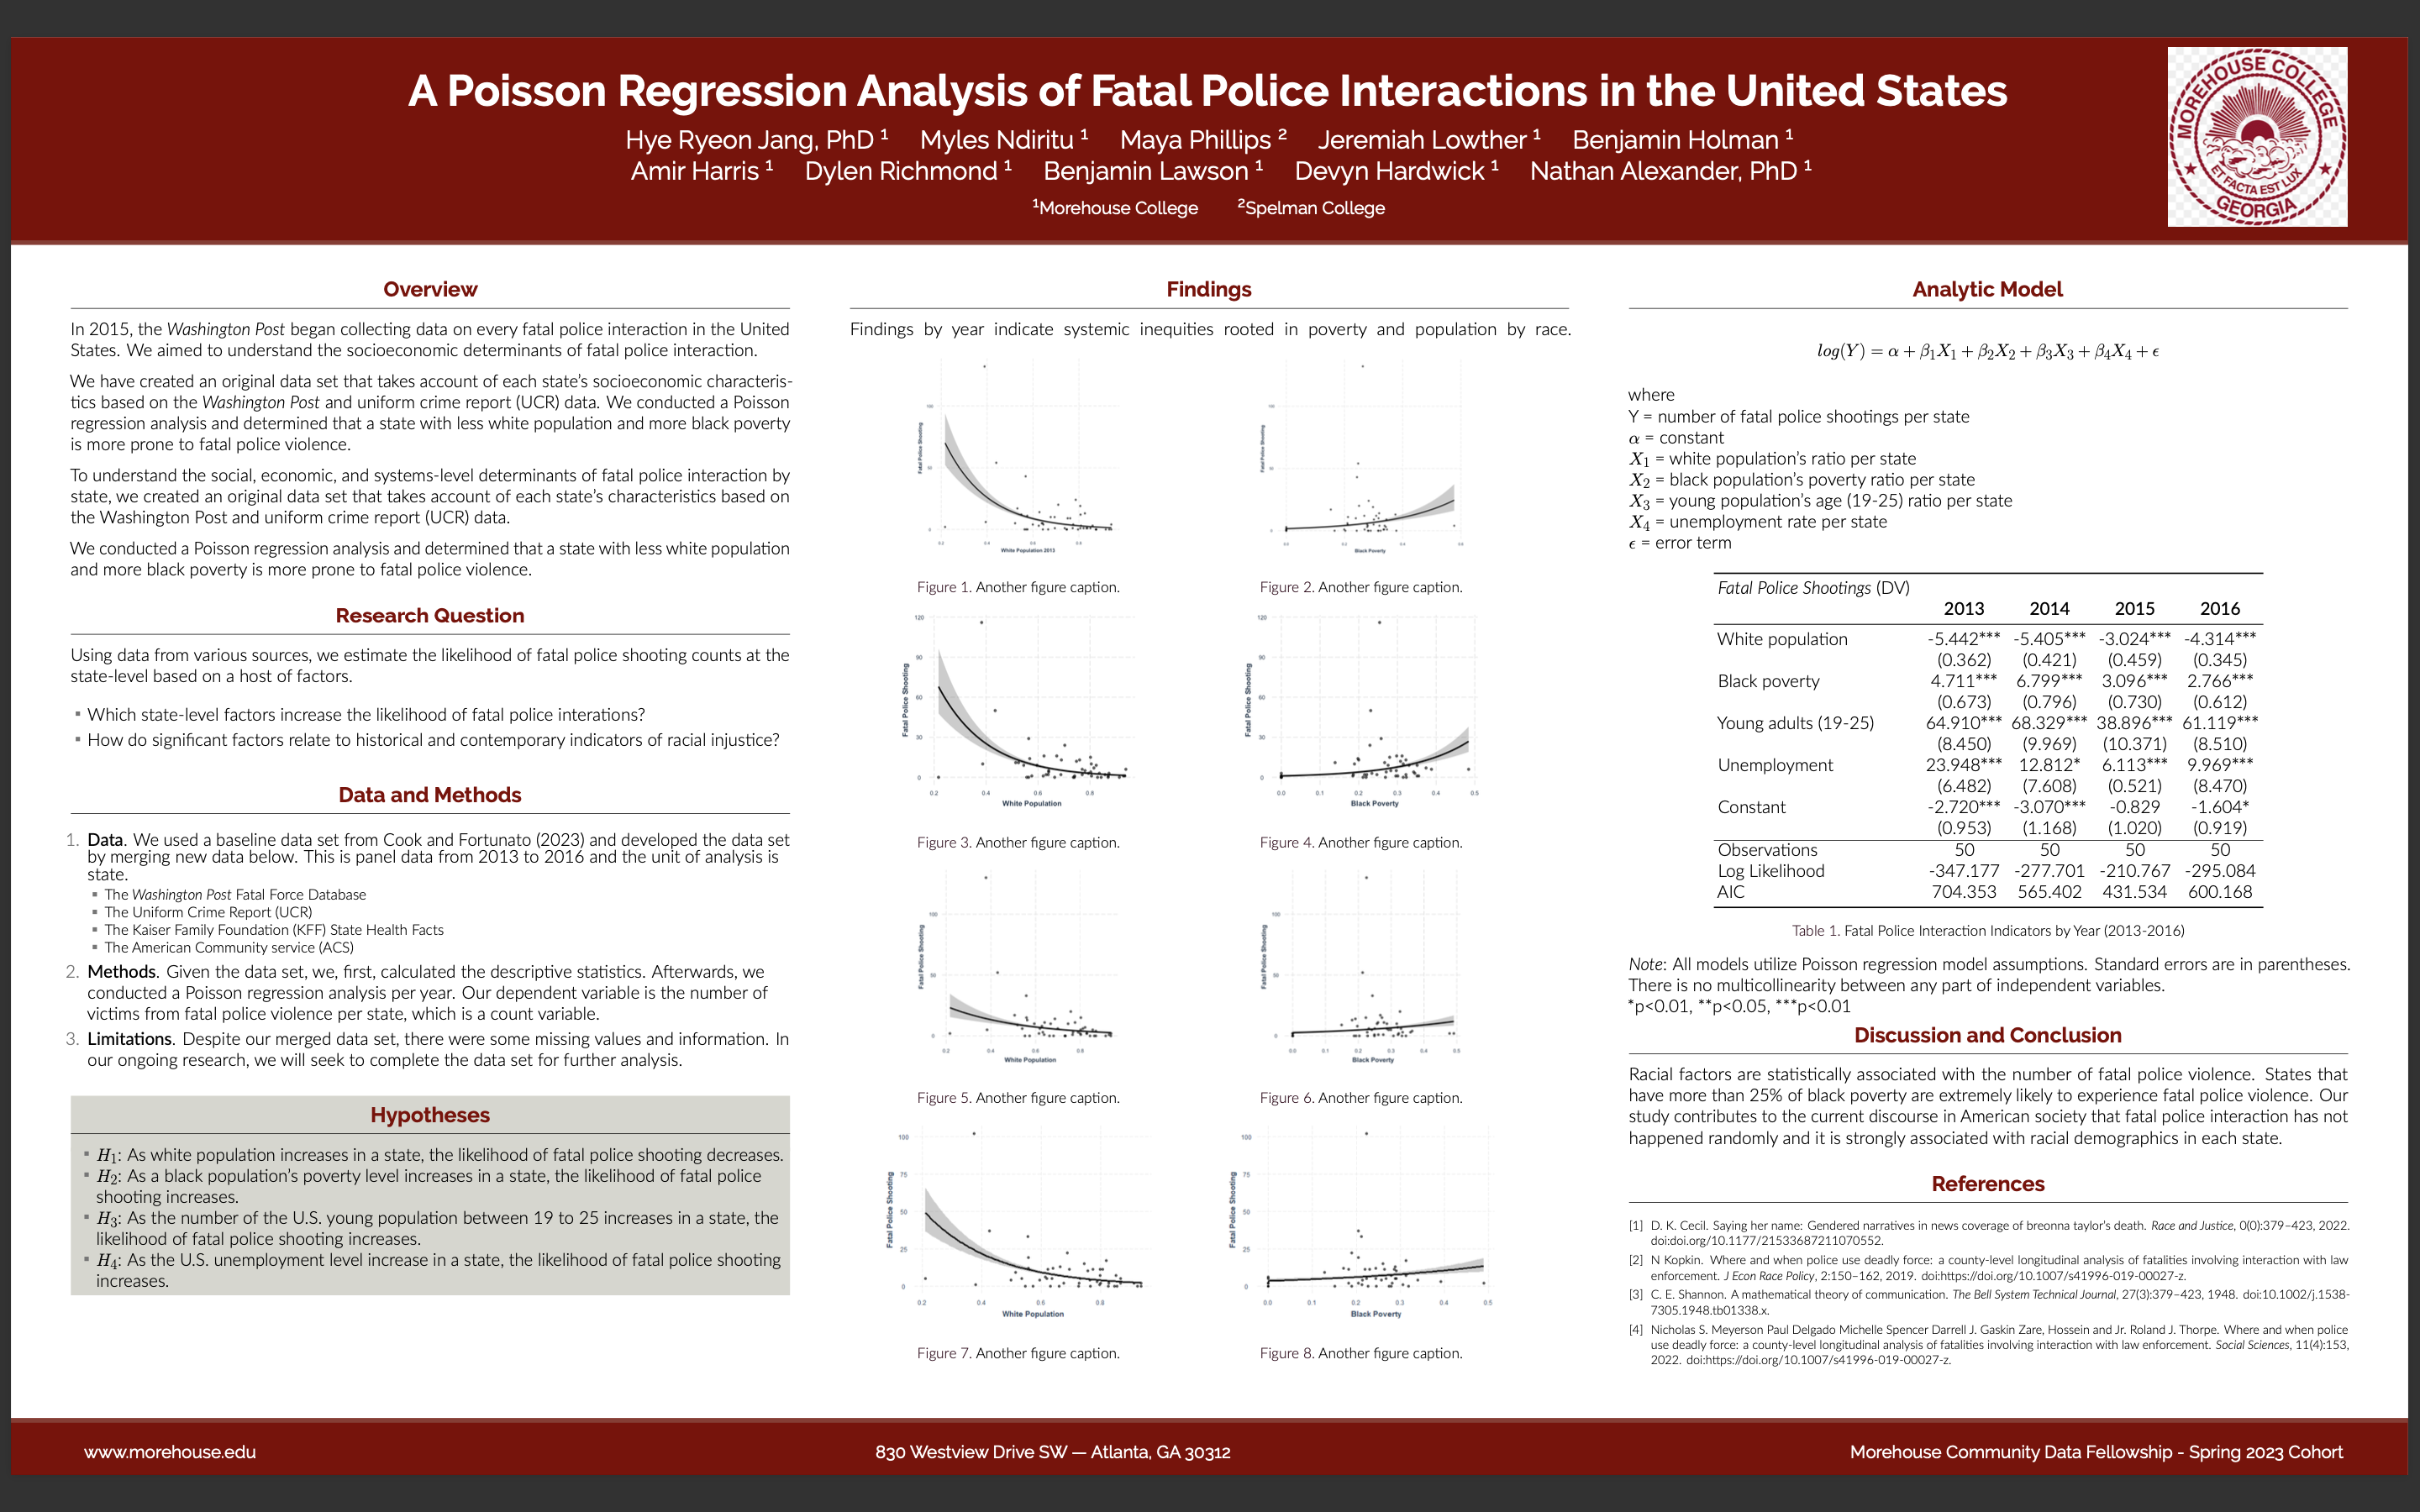
\includegraphics{poster3.png}
\caption{Faculty and student research poster}
\end{figure}
\end{block}

\begin{block}{Campus Policing}
\protect\hypertarget{campus-policing}{}
\end{block}

\begin{block}{Policing on college campuses}
\protect\hypertarget{policing-on-college-campuses}{}
\begin{itemize}[<+->]
\item
  Background

  \begin{itemize}[<+->]
  \item
    First recorded instance of police officers on Yale University's
    campus in 1894
  \item
    An overwhelming 95\% of college campuses employ campus police
    officers (Davis, 2023)
  \item
    Black student voices continue to elevate issues with campus policing
    (Davis, 2023)
  \end{itemize}
\item
  Policing of Black bodies

  \begin{itemize}[<+->]
  \item
    The history of institutionalized punishment and the legitimization
    of force against Black bodies is ingrained in the fabric of American
    history (Hattery \& Smith, 2017).
  \item
    Case Law: 1938 - \emph{Missouri ex rel.--Gaines vs.~Canada} (Ware,
    2008); 1983 - \emph{Boyle v. Torres} (Warner, Norcross, \& Judd,
    2015)
  \item
    Mental health challenges
  \end{itemize}
\item
  Safety through legislation?

  \begin{itemize}[<+->]
  \item
    Clergy Act of 1990
  \item
    2020 - 119 Bills introduced across 33 states addresing campus safety
    (Villalobos, 2020)
  \item
    Mounting state and local legislation authorizing firearms on college
    campuses.
  \item
    Need for consensus on protection versus imperilment
  \end{itemize}
\end{itemize}
\end{block}

\begin{block}{Policing on college campuses}
\protect\hypertarget{policing-on-college-campuses-1}{}
\begin{figure}
\centering
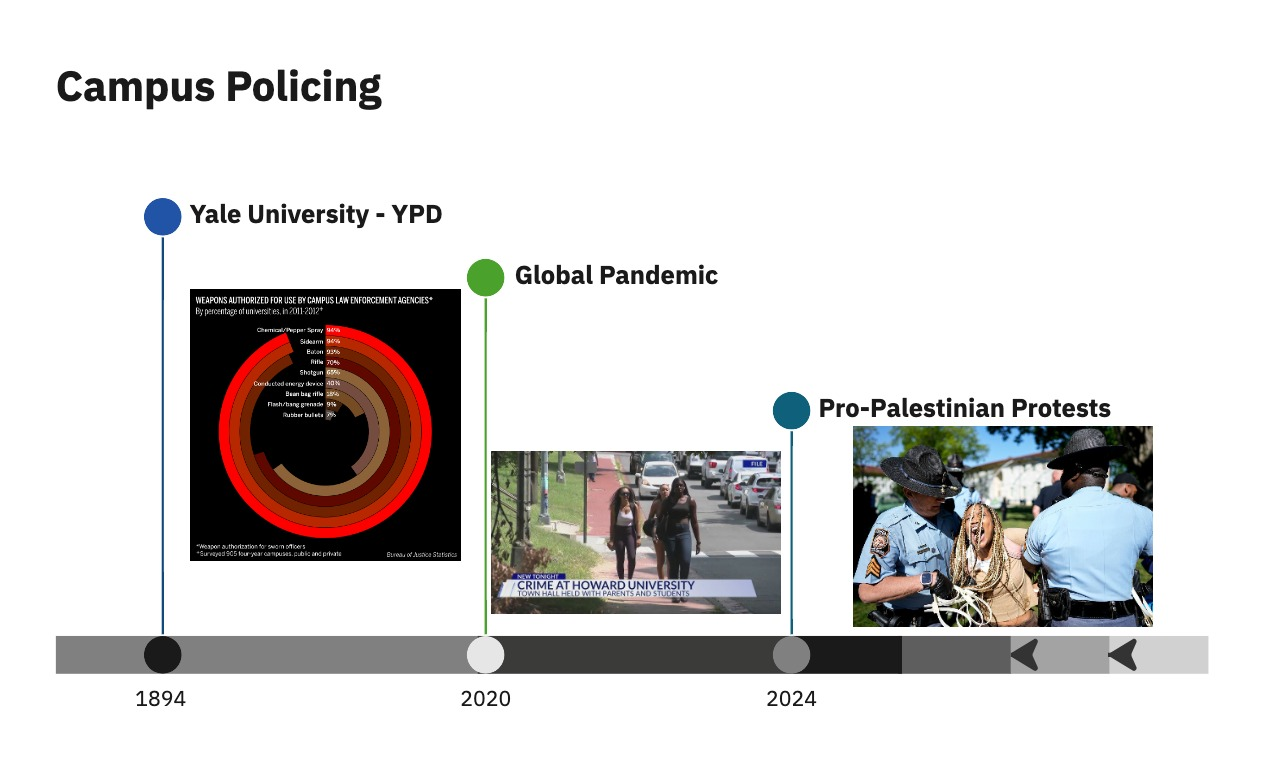
\includegraphics[width=0.25\textwidth,height=\textheight]{campus-policing-timeline.jpg}
\caption{Timeline of campus policing}
\end{figure}
\end{block}

\begin{block}{Prisons}
\protect\hypertarget{prisons}{}
\begin{itemize}[<+->]
\item
  ``In 2021, Black Americans were imprisoned at 5.0 times the rate of
  whites, while American Indians and Latinx people were imprisoned at
  4.2 times and 2.4 times the white rate, respectively.''
  (\href{https://www.sentencingproject.org/reports/one-in-five-ending-racial-inequity-in-incarceration/}{The
  Sentencing Project}, 2023)
\item
  ``One in five Black men born in 2001 is likely to experience
  imprisonment within their lifetime, a decline from one in three for
  those born in 1981. Pushback from policymakers threatens further
  progress in reducing racial inequity in incarceration.''
  (\href{https://www.sentencingproject.org/reports/one-in-five-ending-racial-inequity-in-incarceration/}{The
  Sentencing Project}, 2023)
\end{itemize}
\end{block}

\begin{block}{Prisons}
\protect\hypertarget{prisons-1}{}
The U.S. Bureau of Justice Statistics maintains records of federal and
state prison populations\footnote<.->{Source:
  \href{https://bjs.ojp.gov/library/publications/prisoners-2021-statistical-tables}{Carson
  (2022). Prisoners in 2021 -- Statistical tables. Bureau of Justice
  Statistics.}}.

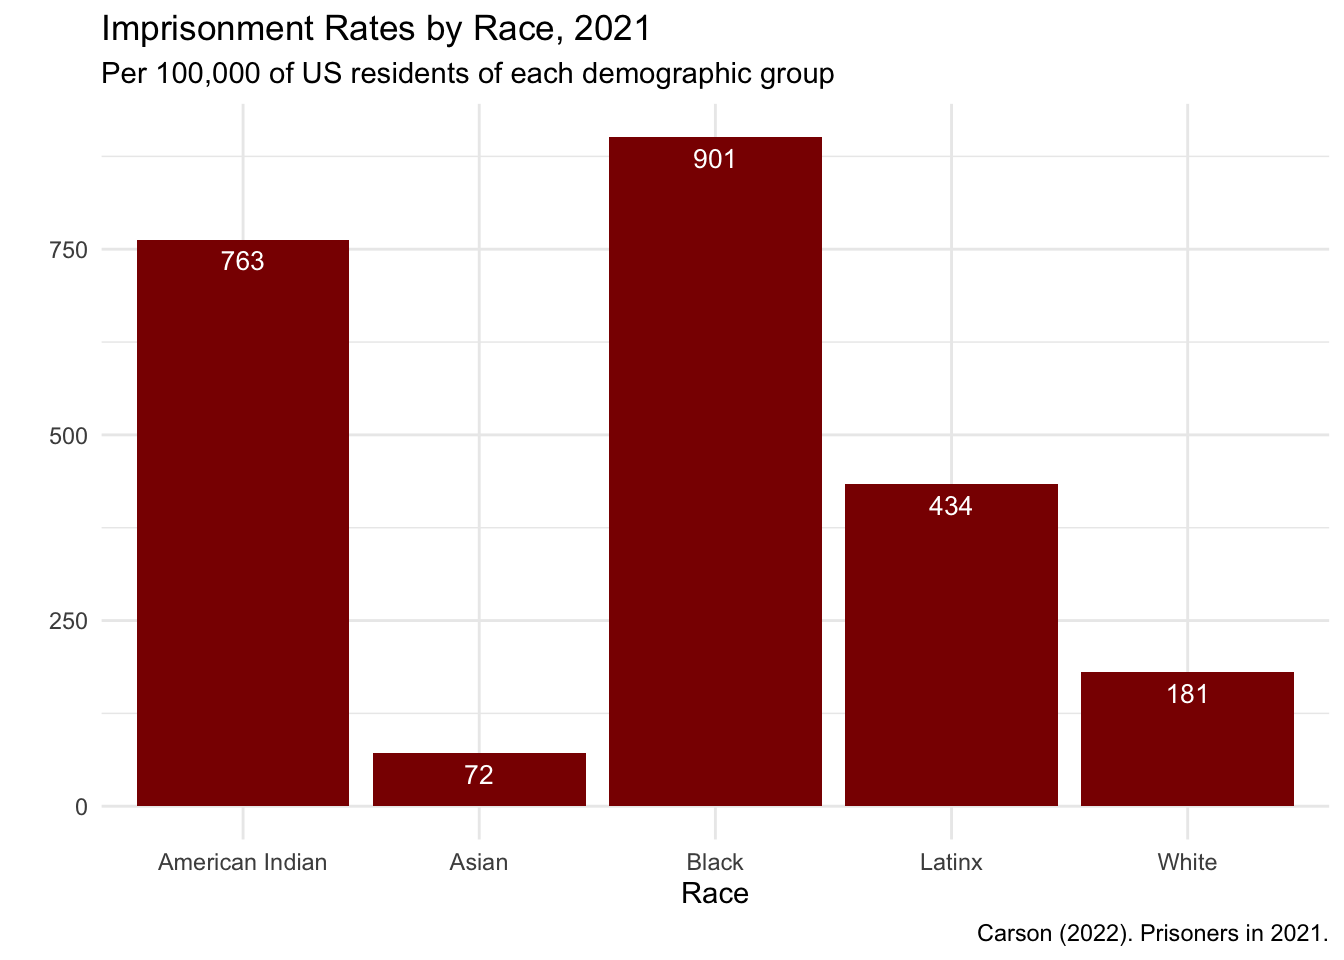
\includegraphics{2024_04_27_bob_moses_files/figure-beamer/unnamed-chunk-7-1.pdf}
\end{block}

\begin{block}{Prisons}
\protect\hypertarget{prisons-2}{}
To support our framing of contemporary data, we take on an historical
view.

\begin{verbatim}
## Rows: 123 Columns: 6
## -- Column specification --------------------------------------------------------
## Delimiter: ","
## chr  (1): Prison Type
## dbl  (4): Total, Total Percentage, White Percentage, Black Percentage
## date (1): Year
## 
## i Use `spec()` to retrieve the full column specification for this data.
## i Specify the column types or set `show_col_types = FALSE` to quiet this message.
\end{verbatim}

\begin{block}{Federal}
\protect\hypertarget{federal}{}
Federal racialization data

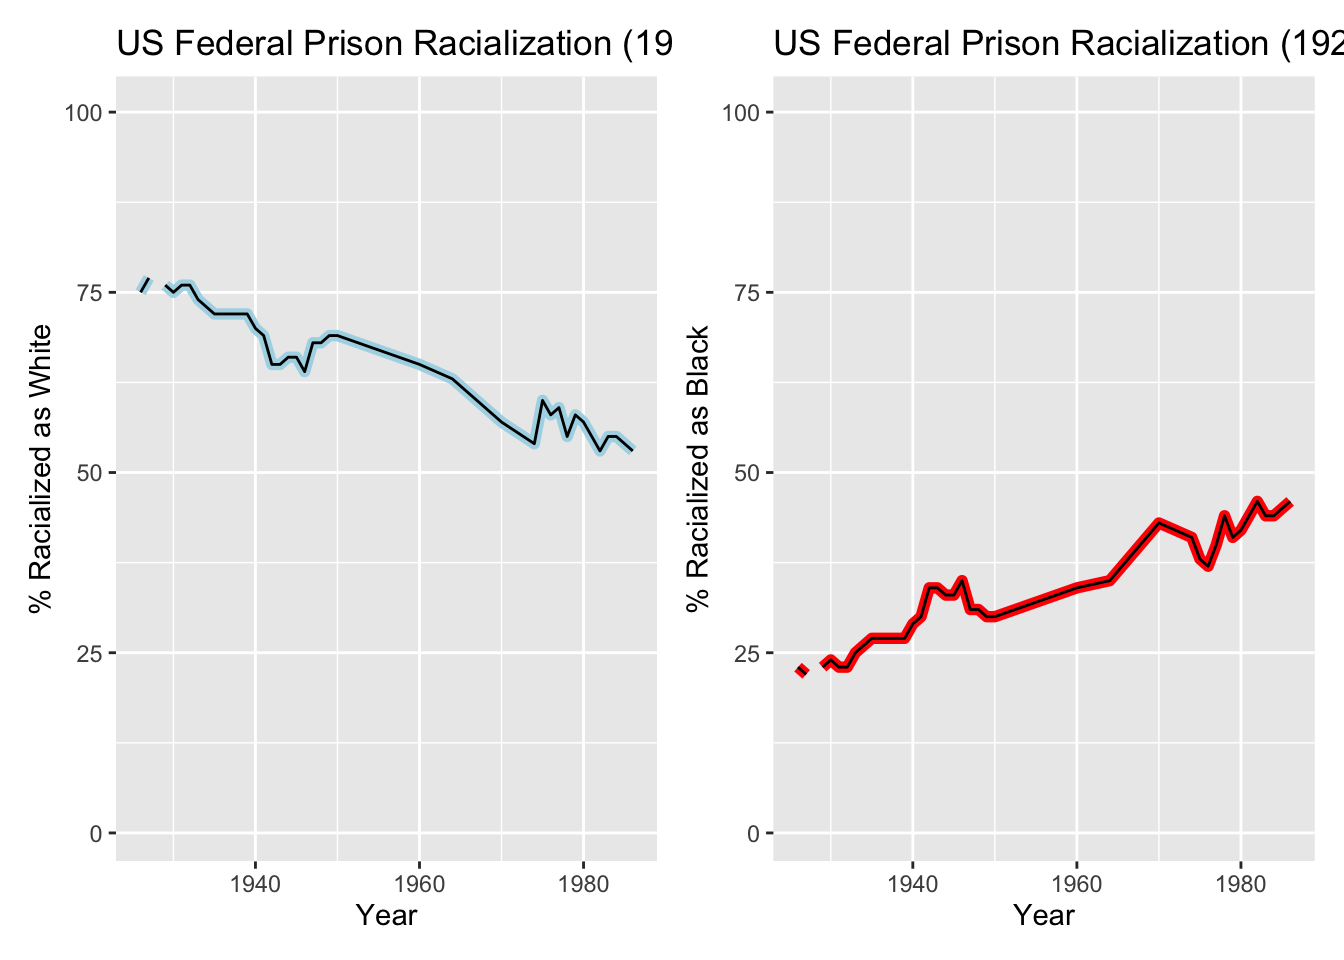
\includegraphics{2024_04_27_bob_moses_files/figure-beamer/unnamed-chunk-10-1.pdf}
\end{block}

\begin{block}{State}
\protect\hypertarget{state}{}
State racialization data

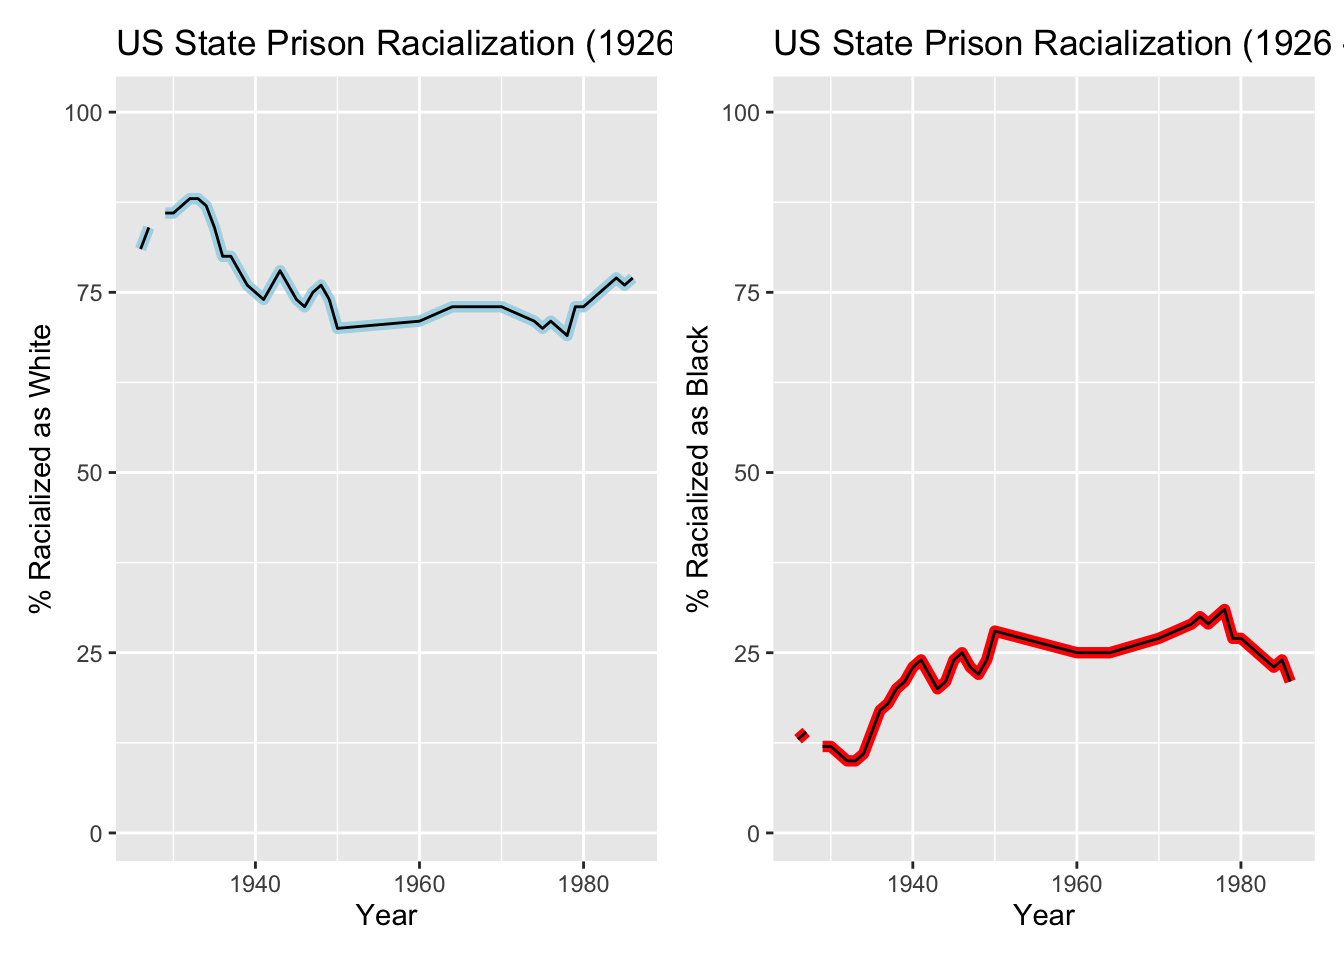
\includegraphics{2024_04_27_bob_moses_files/figure-beamer/unnamed-chunk-12-1.pdf}
\end{block}

\begin{block}{Federal and State}
\protect\hypertarget{federal-and-state}{}
Federal and State racialization data

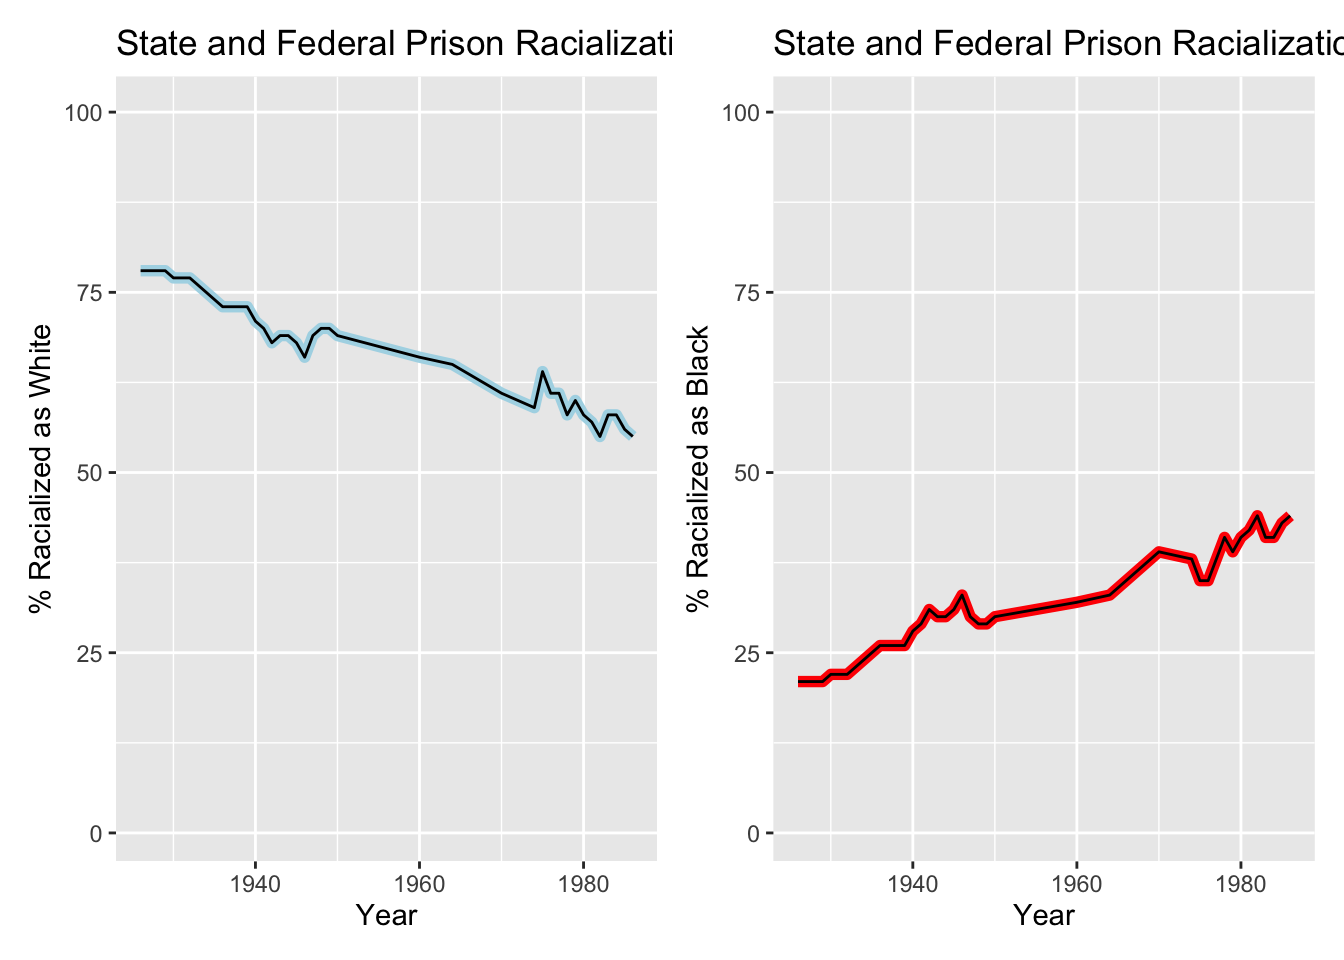
\includegraphics{2024_04_27_bob_moses_files/figure-beamer/unnamed-chunk-14-1.pdf}
\end{block}
\end{block}

\begin{block}{Racism vs.~Anti-Blackness}
\protect\hypertarget{racism-vs.-anti-blackness}{}
In a 2020 NY Times article, kihana miraya ross chronicles the realities
of anti-Blackness.
\href{https://www.nytimes.com/2020/06/04/opinion/george-floyd-anti-blackness.html}{ross
(2020)} deals with the related but differing functions of racism and
anti-Blackness.

\begin{itemize}[<+->]
\item
  ross notes that ``\,`racism' fails to fully capture what black people
  in this country are facing.''
\item
  ross continues by noting that ``Anti-blackness is one way some black
  scholars have articulated what it means to be marked as black in an
  anti-black world.''
\item
  Broadly, ross defines anti-Blackness as society's inability to
  recognize Black people's humanity.
\end{itemize}
\end{block}
\end{frame}

\begin{frame}{Broad Implications}
\protect\hypertarget{broad-implications}{}
\begin{itemize}
\item
  K-12 teaching and learning

  \begin{itemize}
  \tightlist
  \item
    This also exposes students to a diversity of problems and methods to
    solve those problems.
  \end{itemize}
\item
  Computationally-focused research and training in higher education

  \begin{itemize}
  \tightlist
  \item
    Provides an equitable pathway and entry into ``high information,
    high density'' conversations.
  \end{itemize}
\item
  Industry and professional organizations
\end{itemize}
\end{frame}

\begin{frame}{Gratitude for your time.}
\protect\hypertarget{gratitude-for-your-time.}{}
\pause

Thank you for joining us and citing today's presentation.

Alexander, N., Davis, K., Ghali, B., Stewart, Q., \& La Cour, G. (2024,
April 26). The Principles of Reconstruction: Still a Viable Route to
Full Citizenship. \emph{The 2024 Bob Moses Conference}.
\href{https://www.bobmosesconference.com/}{Online}.
\end{frame}

\end{document}
